% Compile with:
% latexmk -lualatex -pvc -interaction=nonstopmode 20220629_MICResearchDay.tex
%\documentclass[aspectratio=169,draft]{beamer}
\documentclass[aspectratio=169]{beamer}
\usetheme{UniBern}

\title{micro-CT imaging across scales and faculties}
\author{David Haberthür}
\date{June 29, 2022 | \href{https://www.mic.unibe.ch/events/mic_research_day_2022}{MIC Research Day 2022}}

\includeonlyframes{current}
%then....
%\begin{frame}[label=current]
%\end{frame}

\usepackage[detect-all=true,
	per-mode=symbol,
	per-symbol=/]{siunitx}
\usepackage{xspace}
\usepackage{gitinfo2}
\usepackage[backend=biber,
	style=numeric,
	url=false,
	maxnames=1,
	sorting=none,
	]{biblatex}
\addbibresource{/home/habi/P/Documents/library.bib} % anaklin25
%\addbibresource{/Users/habi/Documents/library.bib} % anomalocaris
\usepackage{ccicons}
\usepackage{animate}
\usepackage{tikz}
	\usetikzlibrary{spy,shadows,mindmap}
	\tikzset{shadowed/.style={preaction={transform canvas={shift={(1pt,-1pt)}},draw=ubRed}}}
\usepackage{shadowtext} % for the shadowed scalebar
	\shadowoffset{1pt}
	\shadowcolor{ubRed}
\usepackage[absolute,overlay]{textpos} % for the \source* command
\usepackage{fontawesome5}
\usepackage{emoji}
\usepackage{listings}
	\lstset{frame=single,
	basicstyle=\tiny\ttfamily
	}
\usepackage{booktabs}
\usepackage{multirow}
\usepackage{colortbl}
\usepackage{adjustbox}
\usepackage{microtype}

% Some often used abbreviations/commands
\newcommand{\everyframe}{25} % use only every nth frame for the animations
\newcommand{\imwidth}{\linewidth}% set global image width
\newcommand{\imheight}{0.725\paperheight}% set global image height
\newlength\imagewidth% needed for scalebars
\newlength\imagescale% needed for scalebars
\newcommand{\uct}{\textmu CT\xspace}% make our life easier
\newcommand{\eg}{e.\,g.\xspace}%
\newcommand{\ie}{i.\,e.\xspace}%

% Define complementary colors to ubRed
\definecolor{ubRedComplementary1}{HTML}{00a1e6}
\definecolor{ubRedComplementary2}{HTML}{00e645}

% Acknowledge images just below them
% Based on https://tex.stackexchange.com/a/282637/828
\newcommand{\source}[2]{%
	% Print out (short) link under image, with small text
	\raisebox{-1.618ex}{%
		\makebox[0pt][r]{%
			\scriptsize\href{http://#1}{#1} #2%
			}%
		}%
	}%
\newcommand{\sourcecite}[2]{%
	% Cite (an image from) a reference
	\raisebox{-1.618ex}{%
		\makebox[0pt][r]{%
			\scriptsize From \cite{#1}, #2%
			}%
		}%
	}%
\newcommand{\sourcelink}[3]{%
	% Make the source command an \href{link}{text}
	\raisebox{-1.618ex}{%
		\makebox[0pt][r]{%
			\scriptsize\href{http://#1}{#2}, #3%
			}%
		}%
	}%

% Define us a custom footer *with* progress bar, based on https://tex.stackexchange.com/a/59749/828
\makeatletter
\def\progressbar@progressbar{} % the progress bar
\newcount\progressbar@tmpcounta% auxiliary counter
\newcount\progressbar@tmpcountb% auxiliary counter
\newdimen\progressbar@pbht %progressbar height
\newdimen\progressbar@pbwd %progressbar width
\newdimen\progressbar@rcircle % radius for the circle
\newdimen\progressbar@tmpdim % auxiliary dimension
\progressbar@pbwd=0.85\linewidth
\progressbar@rcircle=1.5pt
\def\progressbar@progressbar{%
	\progressbar@tmpcounta=\insertframenumber
	\progressbar@tmpcountb=\inserttotalframenumber
	\progressbar@tmpdim=\progressbar@pbwd
	\multiply\progressbar@tmpdim by \progressbar@tmpcounta
	\divide\progressbar@tmpdim by \progressbar@tmpcountb
	\par%
	\begin{tikzpicture}%
		\draw[ubGrey] (0,0) -- ++ (\progressbar@pbwd,0);
		\draw[draw=ubRed,fill=ubGrey] (\the\dimexpr\progressbar@tmpdim-\progressbar@rcircle\relax,.5\progressbar@pbht) circle (\progressbar@rcircle);
	\end{tikzpicture}%
	\hfill bit.ly/MICRday\xspace|\xspace%
	v. \href{https://github.com/habi/Talk.2022.MICResearchDay/commit/\gitHash}{\gitAbbrevHash}\xspace|\xspace%
	p.\xspace\insertframenumber/\inserttotalframenumber%
	\hspace*{4ex}%
	\vspace{0.5ex}%
	%\par%
}
\addtobeamertemplate{footline}{}%
{%
	\begin{beamercolorbox}[wd=\paperwidth,center]{green}%
		\progressbar@progressbar%
	\end{beamercolorbox}%
}%
\makeatother

% Format bibliography for beamer
% http://tex.stackexchange.com/a/10686/828
\renewbibmacro{in:}{}
% http://tex.stackexchange.com/a/13076/828
\AtEveryBibitem{%
	\clearfield{journaltitle}
	\clearfield{pages}
	\clearfield{volume}
	\clearfield{number}
	\clearname{editor}
	\clearfield{issn}
	\clearfield{year}
}
% No parentheses around the (now empty) year: https://tex.stackexchange.com/a/147537/828
\renewcommand{\bibopenparen}{\addcomma\addspace}
\renewcommand{\bibcloseparen}{\addcomma\addspace}

% open in fullscreen
\hypersetup{pdfpagemode=FullScreen}

% Move the whole text area down a bit
% THIS IS A BIG HACK, AND SHOULD BE FIXED IN THE TEMPLATE
\addtobeamertemplate{frametitle}{}{\vspace*{0.71em}}

\begin{document}
% No footline on the title page
% http://tex.stackexchange.com/a/18829/828 helps us to achieve that
{%
	\setbeamertemplate{footline}{}%
	\begin{frame}%
		\maketitle
	\end{frame}%
}

\begin{frame}
	\frametitle{\emph{Grüessech} from the \uct-group}
	\centering
	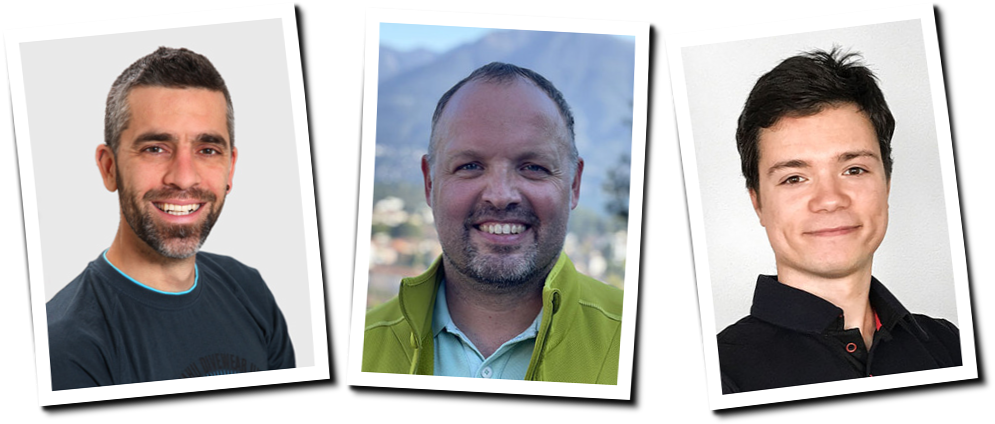
\includegraphics[width=\linewidth]{./images/team}
\end{frame}

\begin{frame}
	\frametitle{LOAFS}
	\uct
	
	Non-destructive imaging across scales
	
	Ich zeige nur \emph{uni-interne} Projekte, wir machen noch (viel) mehr	
\end{frame}

\begin{frame}
	\frametitle{Machinery at the Institute of Anatomy}
	\begin{columns}
		\begin{column}{0.333\linewidth}
			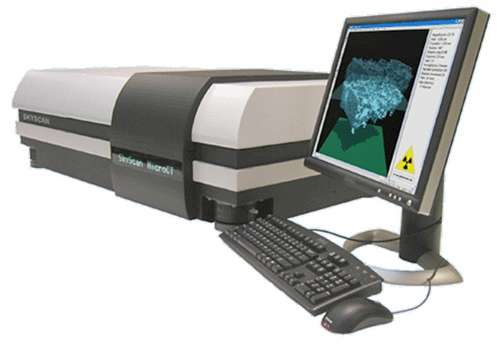
\includegraphics[width=\linewidth]{./images/1172}%
			\source{brukersupport.com}{}
		\end{column}
		\begin{column}{0.333\linewidth}
			\includegraphics<1>[width=\linewidth]{./images/1272}%
			\source{bruker.com/skyscan1272}{}
		\end{column}
		\begin{column}{0.333\linewidth}
			\includegraphics<1>[width=\linewidth]{./images/2214}%
			\source{bruker.com/skyscan2214}{}
		\end{column}							
	\end{columns}
\end{frame}

\tikzset{small mindmap}
%\tikzset{level 1 concept/.append style={level distance = 30mm}}
%\tikzset{level 2 concept/.append style={font=\sf, sibling angle=45,level distance = 17mm}}
%\tikzset{every child/.append style={scale=1.11}}
\tikzset{level 1 concept/.append style={scale=0.9,level distance = 40mm,transform shape}}
\tikzset{level 2 concept/.append style={scale=0.95,level distance = 25mm,transform shape}}
%\tikzset{level 1 concept/.append style={font=\small}}
%\tikzset{level 2 concept/.append style={font=\tiny}}

\begin{frame}[label=current]
	\frametitle{Overview}
	\centering
	\only<1>{
	\begin{tikzpicture}
		\path[mindmap,every node/.style={concept,circular drop shadow},
concept color=ubRed]
			node[concept] {unibe.ch\ Faculties}
				child [grow=15]  {node[concept] {Business, Economics ​and Social Sciences} }
				child [grow=45]  {node[concept] {​Law} }
				child [grow=315] {node[concept] {​Theology}}
				child [grow=135] {node[concept] {​Human Sciences} }
	    			child [grow=165] {node[concept] {​Science} }
	    			child [grow=195] {node[concept] {​Humanities} }				
				child [grow=345] {node[concept] {​Medicine} }
    				child [grow=225] {node[concept] {Vetsuisse} };
	\end{tikzpicture}
	}
	\only<2>{
	\begin{tikzpicture}
		\path[mindmap,every node/.style={concept,circular drop shadow},
concept color=ubRed!31!white,semitransparent]
			node[] {unibe.ch\ Faculties}
			child [grow=-45] {node[concept] {​Theology}}
			child [grow=45]  {node[concept] {​Law} }
			child [grow=15]  {node[concept] {Business, Economics ​and Social Sciences} }
			child [concept color=ubRed,opaque,grow=-15] {node[concept] {​Medicine}
				child [concept color=ubRed,opaque,grow=105]  {node[concept] {Theodor Kocher Institute}}
				child [concept color=ubRed,opaque,grow=140] {node[concept] {School of Dental Medicine}}
				child [concept color=ubRed,opaque,grow=185] {node[concept] {Institute of Anatomy}}
				child [concept color=ubRed,opaque,grow=225] {node[concept] {Klinik für Orthopädische Chirurgie \& Traumatologie}}		
				}
    			child [concept color=ubRed,opaque,grow=225] {node[concept] {Vetsuisse} }
    			child [grow=195] {node[concept] {​Humanities} }
    			child [grow=135] {node[concept] {​Human Sciences} }
    			child [concept color=ubRed,opaque,grow=165] {node[concept] {Science}
				child [concept color=ubRed,opaque,grow=-45] {node[concept] {{Institute of Ecology and Evolution}}}
				child [concept color=ubRed,opaque,grow=15]  {node[concept] {Space Research \& Planetary Sciences}}
    }
    			;
\end{tikzpicture}
}
\end{frame}

\begin{frame}
	\frametitle{Overview}
	% Get emojis from https://unicode.org/emoji/charts/emoji-list.html
	\centering
	\huge
	\emoji{horse} % or \emoji{unicorn} ?
	\emoji{peach}
	\emoji{fish} % or \emoji{tropical-fish} ?
	\emoji{mouse-face}  % or \emoji{mouse} ?
	\emoji{tooth}
	\emoji{nut-and-bolt}
	\emoji{comet}
\end{frame}

\begin{frame}[label=current]
	\frametitle{Overview}
	\begin{columns}
		\begin{column}{0.309\linewidth}
			Scales
			\begin{itemize}
				\item Hoof
				\item Sakrum
				\item Fishes, large to small	
				\item Mouse brain (?)
				\item Teeth
				\item Implants (Straumann, e.g. no faculty)
				\item Chondrules
			\end{itemize}
		\end{column}
		\begin{column}{0.618\linewidth}
			Faculties
			\begin{itemize}
				\item Vetsuisse Faculty
				\item Science
				\begin{itemize}
					\item Institute of Ecology and Evolution
					\item Space Research \& Planetary Sciences (WP)
				\end{itemize}	
				\item Medicine
				\begin{itemize}
					\item Theodor Kocher Institute (TKI)
					\item School of Dental Medicine
					\item Institute of Anatomy
					\item Universitätsklinik für Orthopädische Chirurgie und Traumatologie
				\end{itemize}
			\end{itemize}
		\end{column}
	\end{columns}
\end{frame}

\begin{frame}
	\frametitle{Hoof}
	\begin{columns}
		\begin{column}{0.5\linewidth}
		Laminitis \cite{Blaettler2022}
		Contrast-agent \cite{Hlushchuk2018}
		\end{column}
		\begin{column}{0.5\linewidth}
	\centering
	\animategraphics[height=\imheight,every=\everyframe]{24}{./images/VETSUISSE/HorseLimb/Limb02/setup-frames/IMG_69500}{001}{634}
	\end{column}
		\end{columns}
\end{frame}

\renewcommand{\imwidth}{\imheight}
\begin{frame}
	\frametitle{Hoof}
	\begin{columns}
		\begin{column}{0.5\linewidth}
		\centering
			\pgfmathsetlength{\imagewidth}{\imwidth}%
			\pgfmathsetlength{\imagescale}{\imagewidth/1536}%
			\def\x{949-100}% scalebar-x starting at golden ratio of image width of 1536px = 949
			\def\y{1335}% scalebar-y at 90% of image height of 1483px = 1335
			\def\mag{4}% magnification of inset
			\def\size{75}% size of inset
			\begin{tikzpicture}[x=\imagescale,y=-\imagescale,spy using outlines={rectangle,magnification=\mag,size=\size,connect spies}]
				\node[anchor=north west, inner sep=0pt, outer sep=0pt] at (0,0) {\includegraphics[width=\imagewidth]{./images/VETSUISSE/HorseLimb/Limb02/"MAX_Reslice of merged-bin2x"}};
				%\spy [red] on (666,666) in node at (0,0) [anchor=north west];
				% Since we draw the scale bar on the *binned* dataset, each pixel is not 40.999924, but 81.999848 um
				% 1536.000px = 125.95176652800001mm -> 100px = 8199.985um -> 6.098px = 500um, 1.220px = 100um
				\draw[|-|,blue,thick] (0,742) -- (1536,742) node [sloped,midway,above,fill=white,semitransparent,text opacity=1] {\SI{125.95}{\milli\meter} (1536px) TEMPORARY!};
				\draw[|-|,white,thick,shadowed] (\x,\y) -- (\x+609.8,\y) node [midway,above] {\shadowtext{\SI{5}{\centi\meter}}};
	%\draw[color=red, anchor=south west] (0,1483) node [fill=white, semitransparent] {Legend} node {Legend};
\end{tikzpicture}%
		\end{column}
		\begin{column}{0.5\linewidth}
	\centering
	\animategraphics[palindrome,height=\imheight,every=\everyframe]{24}{./images/VETSUISSE/HorseLimb/Limb02/frames/video-0}{000}{300}
	\end{column}
	\end{columns}
\end{frame}

\begin{frame}
	\frametitle{Sakrum}
	\centering
	\animategraphics[palindrome,height=\imheight,every=\everyframe]{24}{./images/Halm/Becken/Sakrum_C/frames/video-0}{000}{101}
\end{frame}

%\begin{frame}
%	\frametitle{Cichlids}
%	\centering
%	\only<1>{\animategraphics[height=\imheight,every=\everyframe]{24}{./images/EAWAG/161543/head_30um/frames/video-0}{000}{075}}
%	\only<2>{\animategraphics<2>[autoplay,height=\imheight,every=\everyframe]{24}{./images/EAWAG/161543/head_30um/frames/video-0}{075}{240}}
%	\only<3>{\animategraphics<3>[autoplay,height=\imheight,every=\everyframe]{24}{./images/EAWAG/161543/head_30um/frames/video-0}{241}{320}}
%\end{frame}

\begin{frame}
	\frametitle{Thanks}
	Images from us
	
	Werbung für Workshop: COMULIS Training School: \url{https://www.ana.unibe.ch/continuing_education/comulis_training_school/}
\end{frame}

\begin{frame}
	\frametitle{References}
	% Make the references continuously smaller :)
	%\renewcommand*{\bibfont}{\small}
	%\renewcommand*{\bibfont}{\footnotesize}
	%\renewcommand*{\bibfont}{\scriptsize}
	%\renewcommand*{\bibfont}{\tiny}
%	\setbeamertemplate{bibliography item}{\insertbiblabel}
	\printbibliography
\end{frame}

\end{document}
